% MSRI - SGS Sparsity week 1, Tuesday, 2 lectures, 60 minutes each

\documentclass{beamer}

\usepackage{amsmath,amssymb,amsthm,mathrsfs,amscd}
\usepackage{datetime}
\usepackage{csquotes}
\usepackage{hyperref}
\usepackage{graphicx}
\usepackage{tikz,tikz-cd}
\usetikzlibrary{arrows,shapes}

\usetheme{Metropolis}
\metroset{block=fill}



\newcounter{maincounter}
\newcounter{excounter}

\newtheorem{conjecture}{Conjecture}
% \setbeamercolor{block body}{bg=mDarkTeal!15}
% \setbeamercolor{block title}{bg=mDarkTeal,fg=black!2}


\newcounter{maincounter}
\newcounter{excounter}
\numberwithin{maincounter}{chapter}
\numberwithin{equation}{chapter}
\numberwithin{excounter}{chapter}
\renewcommand{\theexcounter}{\thechapter.\Alph{excounter}}
\newtheorem{lemma}[maincounter]{Lemma}
\newtheorem{proposition}[maincounter]{Proposition}
\newtheorem{corollary}[maincounter]{Corollary}
\newtheorem{remark}[maincounter]{Remark}
\newtheorem{theorem}[maincounter]{Theorem}
\newtheorem{exercise}[excounter]{Exercise}
\newtheorem{example}[maincounter]{Example}

\newtheorem*{crucial}{Crucial Observation}

\newtheorem{conjecture}[maincounter]{Conjecture}
\newtheorem{definition}[maincounter]{Definition}

\def\AA{\mathbb{A}}
\def\BB{\mathbb{B}}
\def\EE{\mathbb{E}}
\def\HH{\mathbb{H}}
\def\DD{\mathbb{D}}
\def\NN{\mathbb{N}}
\def\RR{\mathbb{R}}
\def\TT{\mathbb{T}}
\def\CC{\mathbb{C}}
\def\ZZ{\mathbb{Z}}
\def\PP{\mathbb{P}}
\def\QQ{\mathbb{Q}}
\def\FF{\mathbb{F}}
\def\GG{\mathbb{G}}
\def\LL{\mathbb{L}}
\def\MM{\mathbb{M}}
\def\SS{\mathbb{S}}
\def\UU{\mathbb{U}}
\def\XX{\mathbb{X}}


%%% Philipp's macros

\newcommand{\dom}[1]{{\mathrm {dom}}({#1})}
\newcommand{\sman}[1]{{#1}^{\mathrm{sm,an}}}
\newcommand{\ansm}[1]{{#1}^{\mathrm{an,sm}}}
\newcommand{\sm}[1]{{#1}^{\mathrm{sm}}}
\newcommand{\anE}{\mathrm{an}}
\newcommand{\an}[1]{{#1}^{\anE}}
\newcommand{\stab}[1]{{\mathrm{Stab}(#1)}}


\newcommand{\hgtexp}{S}

\newcommand{\rank}{{\rm rank}\,}
\newcommand{\Hpoly}[2]{{H^{}_{#1}({#2})}}
\newcommand{\poly}[2]{{#1^{}({#2})}}
\newcommand{\polyt}[2]{{#1^{\sim}({#2})}}
\newcommand{\polytiso}[2]{{#1^{\sim,{\rm iso}}({#2})}}
%\renewcommand{\graph}[1]{\Gamma({#1})}
\newcommand{\atopx}[2]{{\genfrac{}{}{0pt}{}{#1}{#2}}}
\newcommand{\IP}{{\PP}}
\newcommand{\IG}{{\GG}}
\newcommand{\IH}{{\HH}}
\newcommand{\IC}{{\CC}}
\newcommand{\IR}{{\RR}}
\newcommand{\IT}{{\TT}}
\newcommand{\IRan}{{{\RR}_{\rm an}}}
\newcommand{\IRanexp}{{{\RR}_{\rm an,exp}}}
\newcommand{\RRan}{{\IRan}}
\newcommand{\RRanexp}{{\IRanexp}}
\newcommand{\IRalg}{{\RR}_{\rm alg}}
\newcommand{\IQbar}{{\overline{\QQ}}}
\newcommand{\Kbar}{{\overline{K}}}
\newcommand{\IZ}{{\ZZ}}
\newcommand{\IN}{{\NN}}
\newcommand{\IA}{{\AA}}
\newcommand{\IQ}{{\QQ}}
\newcommand{\IQpbar}{{\overline{\QQ}_p}}
\newcommand{\IQp}{{\QQ_p}}
\newcommand{\ts}[1]{{T}_0({#1})}

\newcommand{\cC}{{\mathcal C}}
\newcommand{\cE}{{\mathcal E}}
\newcommand{\cF}{{\mathcal F}}
\newcommand{\cK}{{\mathcal K}}
\newcommand{\cL}{{\mathcal L}}
\newcommand{\cM}{{\mathcal M}}
\newcommand{\cO}{{\mathcal O}}
\newcommand{\cV}{{\mathcal V}}
\newcommand{\cW}{{\mathcal W}}
\newcommand{\cX}{{\mathcal{X}}}
\newcommand{\cY}{{\mathcal Y}}
\newcommand{\cZ}{{\mathcal Z}}



\newcommand{\defZ}{Z}
\newcommand{\defF}{F}
\newcommand{\defW}{W}
\newcommand{\defC}{C}
\newcommand{\defE}{E}
%\newcommand{\deffam}{F}


\newcommand{\re}[1]{{\rm Re}({#1})}
\newcommand{\imS}{{\rm Im}}
\newcommand{\im}[1]{\imS({#1})}
\newcommand{\imageS}{{\rm im}}
\newcommand{\image}[1]{\imageS({#1})}
\newcommand{\volS}{{\rm vol}}
\newcommand{\vol}[1]{\volS({#1})}
\newcommand{\orth}[1]{{#1}^{\bot}}
\newcommand{\mat}[2]{{\rm Mat}_{#1}({#2})}
\newcommand{\ssm}{\setminus}
\newcommand{\ord}[1]{{\rm ord}({#1})}
\newcommand{\opt}[2]{{\rm Opt}_{#2}({#1})}
\newcommand{\Height}[1]{{H}({#1})}
\newcommand{\trdeg}{{\rm trdeg\,}} 
\newcommand{\geo}[1]{\langle {#1}\rangle_{{\rm geo}}}
\newcommand{\defect}{\delta}
\newcommand{\geodef}{{\delta_{\rm geo}}}
\newcommand{\en}[1]{{\rm End}({#1})}
\newcommand{\Hom}[1]{{\rm Hom}({#1})}
\newcommand{\hommaxR}[1]{\text{\rm Hom}({#1})^{*}_{\IR}}
\newcommand{\arith}{\rm arith}
\newcommand{\sgu}[2]{{#1}^{[{#2}]}}
\newcommand{\oa}[1]{{#1}^{\rm oa}}
\newcommand{\codim}{{\rm codim}}
\newcommand{\lgo}{LGO}
\newcommand{\zcl}[1]{{\rm Zcl}({#1})}


\newcommand{\trans}[1]{{#1}^{T}}

\newcommand{\red}[1]{\textcolor{red}{#1}}

\renewcommand{\subset}{\subseteq} %%% Some people think \subset
%%% excludes equality
\renewcommand{\supset}{\supseteq}

\newcommand{\gra}[1]{\mathrm{Gr}({#1})}


\newcommand{\gl}[2]{{\mathrm {GL}}_{#1}({#2})}
\renewcommand{\sp}[2]{{\mathrm {Sp}}_{#1}({#2})}
\newcommand{\autS}{{\mathrm {Aut}}}
\newcommand{\aut}[1]{\autS({#1})}

\newcommand{\spec}[1]{\mathrm{Spec}\,{#1}}

\newcommand{\tor}[1]{{#1}_{\mathrm{tor}}}
\newcommand{\gal}[1]{{\mathrm{Gal}}({#1})}


\newcommand{\zeroset}[1]{\mathscr{Z}({#1})}


\newcommand{\jac}{\mathrm{Jac}}

\newcommand{\bfzeta}{{\boldsymbol{\zeta}}}

\newcommand{\mattt}[4]
{\left(
  \begin{array}{cc}
    {#1} & {#2} \\ {#3} & {#4} 
  \end{array}
\right)}

\newcommand{\matto}[2]
{\left(
  \begin{array}{c}
    {#1} \\ {#2}
  \end{array}
\right)}

\newcommand{\matot}[2]
{\left(
  \begin{array}{cc}
    {#1} & {#2}
  \end{array}
\right)}


\title{MSRI Summer Graduate School \\ Sparsity of Algebraic Points \\
  Day 2: O-minimal Geometry}
\author{Philipp~Habegger \\ University of Basel \\ \texttt{philipp.habegger@unibas.ch}}
\date{Tuesday, June 8, 2021}

\begin{document}

\setlength{\abovecaptionskip}{0pt} 
\setlength{\belowcaptionskip}{0pt} 

\renewcommand{\figurename}{Fig.}


\begin{frame}
  \titlepage
\end{frame}

\section{Introduction}
\begin{frame}{O-minimal Geometry}
  \begin{minipage}{0.3\linewidth}
    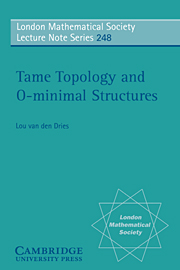
\includegraphics[width=0.9\textwidth]{vddries_title.jpg}    
  \end{minipage}\begin{minipage}{0.6\linewidth}
    O-minimal geometry was developed in the 1980s by various authors
    including Pillay, Steinhorn, and van den Dries. van den Dries called it an
    incarnation of Grothendieck's vision of a ``topologie
    mod\'er\'ee'' (a ``tame topology'') described
    in his ``Esquisse d'un Programme''.  
  \end{minipage}

  ``O'' stands for ``order'',  ``minimal'' is a concept from model
  theory.
\end{frame}

\begin{frame}{Real semi-algebraic sets} 
  O-minimal geometry generalizes real semi-algebaic geometry. 

  \begin{definition}
    A \alert{real semi-algebraic} subset of $\IR^m$ is a finite union
    of sets    
    \begin{equation*}
      \{x\in\IR^m :f_1(x) =\cdots = f_k(x) = 0 \text{ and }
      g_1(x)>0,\ldots,g_l(x)>0\}
    \end{equation*}
    where $f_1,\ldots,f_k,g_1,\ldots,g_l\in \IR[X_1,\ldots,X_m]$.
  \end{definition}

  \begin{example}
    \begin{enumerate}
    \item [(i)] The circle $\{(x,y)\in\IR^2: x^2+y^2=1\}$ is
      real semi-algebraic.
    \item[(ii)] The open disk $\{(x,y) \in\IR^2 : 1-(x^2+y^2)>0\}$ is
      real semi-algebraic and so is the closed disk.
    \item[(iii)] Intervals such as
      $[0,1],[0,1),(0,1],(0,1),(0,\infty),(-\infty,0]$ etc. are real
      semi-algebraic. 
    \end{enumerate}
  \end{example}
\end{frame}

\section{O-minimal Structures}

\begin{frame}{Structures}
  There are two equivalent
  points of view to o-minimal geometry.

  A \alert{structure} is a class of
    subsets of $\IR^m$ \ldots
  \begin{itemize}
  \item \ldots  that are stable under basic operations
    such as: \alert{intersection} $X\cap Y$, \alert{complement}
    $\IR^m\ssm X$,
    \alert{projections} $\pi(X)$, \alert{cartesian products} $X\times
    Z$ and that contain all real semi-algebraic subsets of $\IR^m$.

  \item \ldots that can be defined using certain formulas in
    first-order
    logic, \textit{e.g.}, 
    $\exists y\in \IR : x=y^2$ describes the set $[0,\infty)$,
    $\phi(x,y)\wedge \psi(x,y)$ describes the set of points
    $(x,y)\in\IR^2$ that satisfy both formulas $\phi(x,y)$ and
    $\psi(x,y)$. 
  \end{itemize}
  We will cover both points of view, but will provide only an informal
  approach to first-order logic.
  
  We work exclusively
  over the reals,  there more general versions.
\end{frame}

\begin{frame}{Definition of a Structure}
  \begin{definition}
    A \alert{structure} $\cS$ is a sequence $(S_m)_{m\in\IN_0}$
    where each $S_m$ is a set of subsets of $\IR^m$ with the following
    properties for all $m\in \IN_0$:
    \begin{enumerate}
    \item [(i)] If $X,Y\in S_m$, then $X\cup Y\in S_m$ and
      $\IR^m\ssm X\in S_m$.
    \item[(ii)] If $X\in S_m$, then $\IR\times X\in S_{m+1}$ and $X\times
      \IR\in S_{m+1}$.
    \item[(iii)] If $X\in S_{m}$ and $\pi\colon
      \IR^{m}\rightarrow\IR^k$ is the projection to $k$ distinct
      coordinates, then 
      $\pi(X)\in S_k$.
    \item[(iv)] All real semi-algebraic subsets of $\IR^m$ are in
      $S_m$.
    \end{enumerate}
    A subset of  $\IR^m$ is called \alert{definable} in $\cS$ if it
    is a member of $S_m$.
  \end{definition}

\end{frame}

\begin{frame}{The 2 extremes}
  \begin{example}
    \begin{enumerate}
    \item [(i)] Set $S_m$ to be the set of all subsets of $\IR^m$ for
      all $m\ge 0$. Then $(S_m)_m$ is a structure. 
    \item[(ii)]
      Set $S_m$ to be the set of all real semi-algebraic subsets of $\IR^m$
      for all $m\ge 0$. By definition each $S_m$ is closed under taking
      unions. Closedness under intersections is straight-forward. 
      Say $X\in S_m$, we check that $\IR^m \ssm X$. 
      By closedness under union and intersection we may assume that either 
      \begin{equation*}
        X = f^{-1}(0)=\{ x\in\IR^m : f(x) = 0\}
      \end{equation*}
      or
      \begin{equation*}     
        X = f^{-1}((0,\infty))=\{ (x)\in\IR^m : f(x) > 0\}
      \end{equation*}
      for a single $f\in\IR[X_1,\ldots,X_m]$.
    \end{enumerate}
  \end{example}

\end{frame}

\begin{frame}
  \begin{example}[Continued]
    \begin{enumerate}
    \item [(ii)]
      If $X\subset \IR^m$ is semi-algebraic, then so is $X\times \IR$
      and $\IR\times X$. Indeed, just write down equalities and inequalities
      for $X$ and introduce a dummy coordinate for the extra copy of $\IR$.
      So (ii) is satisfied.

      Clearly, (iv) is satisfied.
      
      What about (iii)? The projection of $\{(x,y) \in\IR^2 :
      x^2+y^2=1\}$ to $\IR$ is $[-1,1] = \{1,-1\}\cup
      \{x\in \IR : x+1>0\text{ and }-x+1>0\}$.
    \end{enumerate}
  \end{example}
  
  \begin{theorem}[Seidenberg--Tarski]
    The projection of a real semi-algebraic subset of $\IR^m$ to
    $\IR^n$ (with $n\le m$) is real semi-algebraic. 
  \end{theorem}

  $\Longrightarrow$ The  real semi-algebraic sets constitute a structure.
\end{frame}

\begin{frame}
  \begin{lemma}
    Let $X\subset\IR^m$ and $Y\subset\IR^n$ be definable in a structure  $\cS$.
    \begin{enumerate}   
    \item [(i)] Then $X\times Y$ is definable.
    \item[(ii)] If $m=n$, then $X\cap Y$ is definable.
    \item[(iii)] The image of $X$ under a polynomial map
      $\IR^m\rightarrow \IR^n$ is definable.
    \end{enumerate}
  \end{lemma}
  \begin{proof}
    \vspace{4cm}
    % For (i) note that $X\times Y =  (X\times \IR^n)\cap (\IR^m\times
    % Y)$. For (ii) we need $X\cap Y = \IR^m\ssm ((\IR^m\ssm X)\cup (\IR^m
    % \ssm Y))$.
    % Let $p_1,\ldots,p_n\in\IR[X_1,\ldots,X_m]$ and consider the graph
    % \begin{equation*}
    %   \Gamma = \{(x_1,\ldots,x_m,x_{m+1},\ldots,x_{m+n})\in\IR^{m+n} :
    %   x_{m+i}-p_i(x_1,\ldots,x_m)= 0 \text{ for all }
    %   i\} 
    % \end{equation*}
    % of $p=(p_1,\ldots,p_n)\colon \IR^m\rightarrow\IR^n$. Then $\Gamma$ is
    % semi-algebraic and it is definable in $\cS$. Now $p(X)$ is the
    % projection of $\Gamma \cap (X\times\IR^n)$ to $\IR^n$ and hence also
    % definable. This gives (iii). 
  \end{proof}
\end{frame}

\begin{frame}{Definable Functions}
  \begin{definition}
    Let $\cS$ be a structure and let $X\subset\IR^m$ be a subset.
    A map $f\colon X\rightarrow\IR^n$ is
    called \emph{definable} in $\cS$, if its graph $\Gamma(f) =
    \{(x,f(x)) : x\in X\}\subset\IR^{m+n}$ is definable in $\cS$.
  \end{definition}

  \begin{example} 
    \begin{enumerate}
    \item [(i)] A polynomial map $\IR^m\rightarrow\IR^n$ is
      definable in $\cS$ by the lemma.
    \item[(ii)]  $\IR\ni x\mapsto |x| =\max\{x,-x\}$ is definable in $\cS$.
    \item[(iii)]  $[0,\infty)\ni x\mapsto \sqrt{x}$ is 
      definable in $\cS$.
    \item[(iv)] The domain $X$ and the image $f(X)$ are both definable
      in $\cS$. Just project!
    \end{enumerate}
  \end{example}
\end{frame}

\begin{frame}{The O-minimal Axiom}  
  The definition of structure does not contain
  any clause that ``tempers'' the collection of sets.
  The structure of all subsets of $\IR^m$ contains many ``wild'' sets:
  fractals, (possibly) non-Lebesgue measurable sets, Peano curves are
  definable maps, etc.

  \begin{definition}
    A {structure} $\cS=(S_m)_m$ is call \alert{o-minimal} if
    \begin{enumerate}
    \item [(v)] each 
      element in $S_1$ is a finite union of points and
      open (possibly unbounded) intervals.
    \end{enumerate}
  \end{definition}

  \begin{example}
    What are the real semi-algebraic subsets of $\IR$? 
    The zero locus of $f\in\IR[X]$ is finite or $\IR$. The pre-image
    $f^{-1}((0,\infty))$ is open in $\IR$  with finitely many
    boundary points. So it is a finite union of open intervals.
  \end{example}
\end{frame}

\begin{frame}{Limits of O-minimality}
  \begin{theorem}[Seidenberg--Tarski]
    The collection of real semi-algebraic sets is an o-minimal
    structure. We denote it by $\IRalg$. 
  \end{theorem}

  As the projection of any definable set to $\IR$ is definable, the
  o-minimal axiom (v) imposes a restriction on \emph{all} sets
  ``upstairs'' in $\IR^m$.

  \begin{example}
    \begin{enumerate}
    \item [(i)] The set of all integers $\IZ$ is \alert{not} definable in any
      o-minimal structure. Neither are the rational numbers $\IQ$.
    \item[(ii)] The function $\sin \colon\IR\rightarrow\IR$ is
      \alert{not} definable in any o-minimal structure. 
    \end{enumerate}
  \end{example}
\end{frame}

%\section{Structures and First-Order Logic}
\begin{frame}
  Informally, a formula constructed inductively from  an expression
  such as ``$x\in X$'' where $X$ is definable
  in the structure, or involves
  the basic field operations $+,\cdot,-,/$
  and the constants $0,1$, as well as $>$.
  
  We can combine two formulas $\phi(x)$ and $\psi(x)$:
  \begin{equation*}
    \begin{array}{ll}
      \phi(x) \wedge \psi(x) & \text{$\psi(x)$ and $\phi(x)$ are true}\\
     \phi(x) \vee \psi(x) & \text{$\psi(x)$ or $\phi(x)$  is true}\\
     \neg \phi(x)  & \text{the negation of $\phi(x)$ is true}\\
     \exists x: \phi(x) &\text{there exists $x$ with $\phi(x)$ true}\\
     \forall x: \phi(x) &\text{for all $x$ the expression is $\phi(x)$ true}
    \end{array}
  \end{equation*}

  The free variable $x$ is understood as tuple of elements in the
  \alert{universe}, which equals $\IR$ in our treatment. 
\end{frame}

\begin{frame}{First-Order Logic}
  \begin{example}
    \begin{enumerate}
    \item [(i)] The expression $(x^2+1=0)\vee(x^2-1>0)$ is a valid
      formula in $\IRalg$. It desribes $(-\infty,-1)\cup(1,\infty)$.
    \item[(ii)] Let $X\subset\IR^2$ be definable in $\IRalg$. Then
      $x : \exists y : (x,y)\in X$ is definable in $\IRalg$, it
      describes the projection of $X$ to the first coordinate. 
    \item[(iii)]
      We are not \alert{allowed} to quantify over sets that are not definable in
      the ambient structure. If $\cS$ is any o-minimal
      structure, then $\IZ$ is not definable in $\cS$. So 
      $$\forall x \in\IZ:\forall y\in\IZ :\forall z\in \IZ :
      (xyz=0) \vee \neg(x^n+y^n=z^n)$$
      does not describe a definable set.
      
    \end{enumerate}
  \end{example}
\end{frame}

\begin{frame}{A Dictionary}
  Below $X$ and $Y$ are usually subsets of $\IR^m$ and $x,y$ refer to
  tuples of real numbers. 
  \begin{center}
    \begin{tabular}{c|c|c}
      $X\cap Y$  & $(x\in X)\wedge (x\in Y)$ &
                                                                                                 $x$  free\\
      $\IR^m\ssm X$  &  $\neg(x\in X)$ & $x$ is free \\
      $X\times\IR$  & $x\in X$&
                                                                   $(x,t)$
                                                                    free\\
      $\pi(X)$  &$\exists y : (x,y)\in
                                      X$  & $x$  free
      \\  
      $X\cup Y$ & $( x\in X)\vee (x\in Y)$ &
                                                                                               $x$
                                             free\\
      $\IR\ssm \pi(\IR^2\ssm X)$ & $\forall y : (x,y)\in X$ & $x$
                                                              free,
                                                              here $X\subset\IR^2$
                                             
    \end{tabular}
  \end{center}
  Remember:  any element  lies in the universe $\IR$  ``by default'' in expressions
  such as $\exists x:\phi(x)$ and $\forall x:\phi(x,y)$.
\end{frame}

\begin{frame}
  \begin{lemma}[Constant/Injective Lemma]
    Let $f\colon (0,1)\rightarrow\IR$ be definable in an o-minimal
    structure. There exist $0=x_1<\cdots <x_n =1$
    such that for all $i$ the restriction  $f|_{(x_i,x_{i+1})}$
    is constant or injective. 
  \end{lemma}
  \begin{proof}\renewcommand{\qedsymbol}{}
    \vspace{4.5cm}
  \end{proof}
\end{frame}

\begin{frame}
  \begin{proof}[Proof continued]
    \vspace{7cm}
  \end{proof}
\end{frame}

\begin{frame}{A Uniformity Statement}
  \begin{corollary}
    Let  $f\colon (0,1)\rightarrow
    \IR$ be definable in an o-minimal structure.
    There exists a constant $B=B(f)$ such that the number of connected
    components of $f^{-1}(y)$ is at most $B$. 
  \end{corollary}

  \begin{theorem}[Monotonity Theorem]
    Let $f\colon (0,1)\rightarrow\IR$ be definable in an o-minimal
    structure. There exist $0=x_1<\cdots <x_n =1$
    such that for all $i$ the restriction  $f|_{(x_i,x_{i+1})}$
    is continuous and either constant or strictly monotone.
  \end{theorem}
\end{frame}

\section{The Cell Decomposition Theorem}

\begin{frame}
  Cells are the basic building blocks for definable sets in o-minimal
  structures.

  We first explain what a cell is an then present the Cell
  Decomposition Theorem.
\end{frame}

\begin{frame}{What is a Cell?}
  \begin{definition}
    Let $\cS$ be an o-minimal structure. 
    A \emph{$(0)$-cell} is a singleton in $\IR$. A \emph{$(1)$-cell} is an open
    interval in $\IR$, \textit{i.e.}, a set for the form $(a,b)$ with
    $a,b\in \IR\cup\{\pm\infty\}$ with $a<b$.

    Suppose $m\ge 1$ and we are given a $(i_1,\ldots,i_m)$-cell
    $C\subset\IR^m$
    (with $i_1,\ldots,i_m\in
    \{0,1\}$).  
    \begin{itemize}
    \item A \emph{$(i_1,\ldots,i_m,0)$-cell} is a the graph of a function
      $f\colon C\rightarrow \IR$ that is definable in $\cS$. In
      particular, it lies in $\IR^{m+1}$.
    \item Let $f,g\in \{\text{functions }C\rightarrow \IR \text{ definable
        in $\cS$}\}\cup\{\pm\infty\}$  with $f(x) < g(x)$ for all $x\in C$. 
      Then
      \begin{equation*}
        \{(x,y)\in C\times \IR : f(x) < y <
        g(x)  \}\subset\IR^{m+1}
      \end{equation*}
      is a \emph{$(i_1,\ldots,i_m,1)$-cell}.
    \end{itemize}
  \end{definition}
\end{frame}

\begin{frame}{Drawings of Cells}

  \vspace{7cm}
  An $(i_1,\ldots,i_m)$-cell is homemorphic to $(0,1)^{i_1+\cdots+i_m}$.
\end{frame}

\begin{frame}{Cell Decomposition Theorem}
  \begin{theorem}
    Let $X\subset\IR^m$ be
    definable in an o-minimal structure.
    \begin{enumerate}
    \item [(i)] Then $X$ is a
      finite disjoint union of cells.
    \item[(ii)] Let $f\colon X\rightarrow\IR$ be 
      a definable function. Then $X=C_1\cup\cdots \cup C_r$ for pairwise
      disjoint cells $C_1,\ldots,C_r\subset\IR^m$ such that
      $f|_{C_i}\colon C_i\rightarrow\IR$ is continuous. 
    \end{enumerate}
  \end{theorem}
\end{frame}

\begin{frame}
  \begin{minipage}{0.6\linewidth}
    \begin{lemma}
      Let $X\subset \IR^{n+m}= \IR^{n}\times
      \IR^m$ be definable in an o-minimal structure. For $y\in\IR^n$ we set
      \begin{equation*}
        X_y = \{ x\in\IR^n : (y,x)\in X\},
      \end{equation*}
      which is also definable. 
    \end{lemma}
  \end{minipage}  \begin{minipage}{0.3\linewidth}
  \end{minipage}

  \begin{theorem}[Uniformity Theorem]
    Let $X\subset \IR^{n+m}= \IR^{n}\times
    \IR^m$ be definable in an o-minimal structure.
    There exists $B\in\IR$ such that for all
    $y\in\IR^n$, the number of
    connected components of $X_y$ is at most $B$.
  \end{theorem}  
\end{frame}

\begin{frame}{Dimension}
  \begin{definition}
    Let $X\subset\IR^m$ be definable in an o-minimal
    structure $\cS$. The
    \alert{dimension} of $X$ is
    \begin{equation*}
      \dim X = \max \{i_1+\cdots+i_m: X\text{ contains an
      }(i_1,\ldots,i_m)-cell\}
    \end{equation*}
    if $X\not=\emptyset$ and $\dim \emptyset=-\infty$. So $\dim X \in
    \{-\infty, 0,\ldots,m\}$. 
  \end{definition}

  \vspace{-0.2cm}
  The dimension is \alert{well-behaved}. Immediate properties:
  \begin{itemize}
    \vspace{-0.2cm}
  \item $\dim X = 0  \Leftrightarrow \text{$X$
      is finite and non-empty}$
  \item
        $\text{$Y\subset\IR^m$ definable in $\cS$ with  $X\subset Y$}
        \Rightarrow 
    \dim X\le \dim Y.$
  \end{itemize}
  \vspace{-0.2cm}
  Further properties:  
  \begin{itemize}
      \vspace{-0.2cm}
  \item $X,Y\subset\IR^m$  definable $\Rightarrow \dim X\cup Y = \max\{\dim X,\dim Y\}$.
  \item $X\subset\IR^m,Y\subset\IR^n$  definable $\Rightarrow \dim
    X\times Y = \dim X +\dim Y$.
  \item $X\subset\IR^m$ and $f\colon
    X\rightarrow\IR^n$ is definable, then $\dim f(X) \le \dim X$ with
    equality if $f$ has finite fibers.
  \end{itemize}
\end{frame}

\section{Examples of o-minimal Structures}

\begin{frame}
  The real semi-algebraic sets $\IRalg$ define the smallest possible
  o-minimal structure. For applications to
  number theory it is often not enough. So we present three of the most
  important o-minimal structures.

  \begin{definition}
    Let $\mathscr{X}$ and $\mathscr{F}$ be sets with the following
    properties. For all $X\in \mathscr{X}$ there exists $m\in\IN_0$ with
    $X\subset\IR^m$. For all $f\in \mathscr{F}$ there exists $m\in\IN_0$
    and $X\subset\IR^m$ such that $f$ is a function $X\rightarrow\IR$. The
    \alert{structure generated} by $\mathscr{X},\mathscr{F}$ is the small
    structure in which all elements of $\mathscr{X}$ and $\mathscr{F}$ are
    definable.
  \end{definition}

  \begin{example}
    Let $\IR_{\sin}$ denote the structure generated by
    $\mathscr{X}=\emptyset$ and $\mathscr{F}=\{\sin \}$.
    This structure expands $\IRalg$ but it is no longer o-minimal as
    $\sin^{-1}(0)=\pi\IZ$ is countable infinite.
  \end{example}
\end{frame}

\begin{frame}{Restricted Real Analytic Functions}

  \begin{definition}
    The structure obtained from $\IRalg$ by adjoining
    \begin{alignat*}1
      \mathscr{F} = \{f \colon [0,1]^m\rightarrow\IR:  \,\,&\text{$f$ is the
        restriction of a real analytic}\\&\text{function $U\rightarrow
        \IR$ defined on an}\\
      &\text{open subset
        $U\subset\IR^m$ containing $[0,1]^m$}\}.  
    \end{alignat*}
     is called the structure of \emph{restriced real analytic
       functions}
     and denoted by $\IRan$.
  \end{definition}

  This definition certainly rules out $\sin$ on the full real line.

  \begin{theorem}[Gabrielov]
    The structure $\IRan$ is o-minimal. 
  \end{theorem}
\end{frame}

\begin{frame}{The Compactly Restricted Exponential Function}
  We often identify $\IC$ with $\IR^2$ via
  \begin{equation*}
    \IC\ni z\leftrightarrow (\mathrm{Re}(z),\mathrm{Im}(z))\in\IR^2.
  \end{equation*}
  By extension we often
  identify $\IC^m$ with $\IR^{2m}$ componentwise.

  % Any  map $\IC^m\rightarrow \IC^n$ defined componentwise by complex polynomials in
  % $\IC[X_1,\ldots,X_m]$
  % is real semi-algebraic in these real coordinates.

  \begin{example}
    Under the identification
    $\IC\rightarrow\IR^2$  above
    $\exp\colon\IC\rightarrow\IC$ becomes a real analytic map
    $\IR^2\rightarrow\IR^2$ (\alert{not} definable in any
    o-minimal structure!).
    
    But its restriction to the square $[0,1]^2$ is definable in $\IRan$.
    The restriction ot $\exp$ to any
    closed disk in $\IC$ is definable in $\IRan$.
    \begin{equation*}
      \Rightarrow\{z\in [0,1]^2 : \exp(\exp(z)^2-\exp(z^2)^2)-z^{2021} > \exp(z)\}
    \end{equation*}
    has finitely many connected components.
  \end{example}
\end{frame}

\begin{frame}{Intermezzo on Abelian Varieties}
  We come to an important example in our later applications. 

  Consider an abelian variety $A$
  defined over $\IC$ with $A\subset \IP^n$ and $g=\dim A$.
  Then $A(\IC)$ is a compact complex Lie group. As such there is a
  holomorphic, surjective group homomorphism $u\colon \mathrm{T}_0(A) \rightarrow
  A(\IC)$
  where $\mathrm{T}_0(A)\cong \IC^g$ is the tangent space of $A$ at
  $0$. The \alert{period lattice} is
  \begin{equation*}
    \ker u = \Omega\text{, a discrete rank $2g$ subgroup of $\IC^g$}
  \end{equation*}
  

  We can arrange $u = [\vartheta_0,\ldots,\vartheta_n]$ for theta
  functions $\vartheta_i \colon \IC^g \rightarrow\IC$ that holomorphic
  and $\Omega$-quasi-periodic.
  That is, there is a function $f\colon \IC^g\times \Omega\rightarrow
  \IC^\times$ with 
  \begin{equation}
    \vartheta_i(z+\omega) = f(z,\omega) \vartheta_i(z)
  \end{equation}
  for all $i$, all $z\in\IC^g$, and all $\omega\in\Omega$.
  $\Rightarrow \vartheta_i$ are \alert{not} definable in $\IRan$. 
\end{frame}

\begin{frame}
  Solution: restrict $\vartheta_i$ to a
  \alert{fundamental domain}.
  
  Let $(\omega_1,\ldots,\omega_{2g})$ be a basis of the $\IZ$-module
  $\Omega$. Set
  \begin{minipage}{0.6\linewidth}
    \begin{alignat*}1
      \cF = \{&\lambda_1\omega_1+\cdots+\lambda_{2g}\omega_{2g} :
      \\ &      \lambda_1,\ldots,\lambda_{2g}\in [0,1]\}.
    \end{alignat*}  
  \end{minipage}  \begin{minipage}{0.3\linewidth}
  \end{minipage}

  
  Then $\cF$ is a real semi-algebraic set and in particular definable
  in $\IRan$. 
  Therefore, each \alert{restriction} $\vartheta_i|_{\cF}$ is
  definable in $\IRan$ and
  \begin{equation*}
    u|_{\cF} \colon \cF\rightarrow A(\IC)
  \end{equation*}
  is surjective  with finite fibers.
  This restriction retains enough information on the setting while at
  same time ensures that we can employ o-minimal geometry.
\end{frame}

\begin{frame}
  \begin{lemma}
    Let $V$ be an algebraic subvariety of $A$.
    Then $u|_{\cF}^{-1}(V(\IC))$ is definable in $\IRan$
    of dimension $2\dim V$. 
  \end{lemma}
  \begin{proof}
    \vspace{5cm}
  \end{proof}
\end{frame}

\section{The Exponential Function}

\begin{frame}
  \begin{definition}
    Let $\IRexp$ be the structure generated by
    $\mathfrak{F} = \{ \exp \colon \IR\rightarrow\IR\}$. 
  \end{definition}

This definition involves the exponential function on \alert{full}
{real} line.

\begin{theorem}[Wilkie]
  The structure $\IRexp$ is o-minimal.
\end{theorem}

\begin{example}
  \begin{enumerate}
  \item [(i)]
    The function $(0,\infty)\rightarrow\IR$ given by $x\mapsto \log x$
    is definable in $\IRexp$.
    So is $(0,\infty)\times\IR$ given by $(x,y)\mapsto x^y = \exp(y\log x)$.
  \item[(ii)]The set
      $$\{x\in\IR : \exp(\exp(x)^2-\exp(x^2)^2)-x^{2021} > \exp(x)\}$$
      is a finite union of open intervals.
  \end{enumerate}
\end{example}
\end{frame}

\begin{frame}{Restricted Analytic Functions and the Exponential Function}

  \begin{definition}
    Let $\IRanexp$ be the structure generated by 
    $\IRan$
    and $\exp \colon \IR\rightarrow\IR$.
  \end{definition}

  Anything that is definable in $\IRan$ or $\IRexp$ is also definable
  in  $\IRanexp$.

  \begin{theorem}[van den Dries--Miller]
    The structure $\IRanexp$ is o-minimal.
  \end{theorem}

  $\IRanexp$ is ``big enough'' to treat the Klein's
  modular $j$-function. 
\end{frame}

\begin{frame}{Klein's Modular $j$-function}
   Recall that $j\colon \IH\rightarrow\IC$ is invariant under
    $\mathrm{SL}_2(\IZ)$ and
    $$j(\tau)=q^{-1}+744+196884q+\cdots$$
    with $q = e^{2\pi i \tau}$ and $\tau\in\IH$.

  The action of $\mathrm{SL}_2(\IZ)$ on $\IH$ admits a real semi-algebraic
  fundamental domain
  
  \begin{minipage}{0.5\linewidth}
  \begin{alignat*}1
    \cF = \{ \tau\in \IH: |\tau|\ge 1 \text{ and }
    &|\mathrm{Re}(\tau)|\le 1/2\}
  \end{alignat*}
  \end{minipage} \hfill \begin{minipage}{0.35\textwidth}
    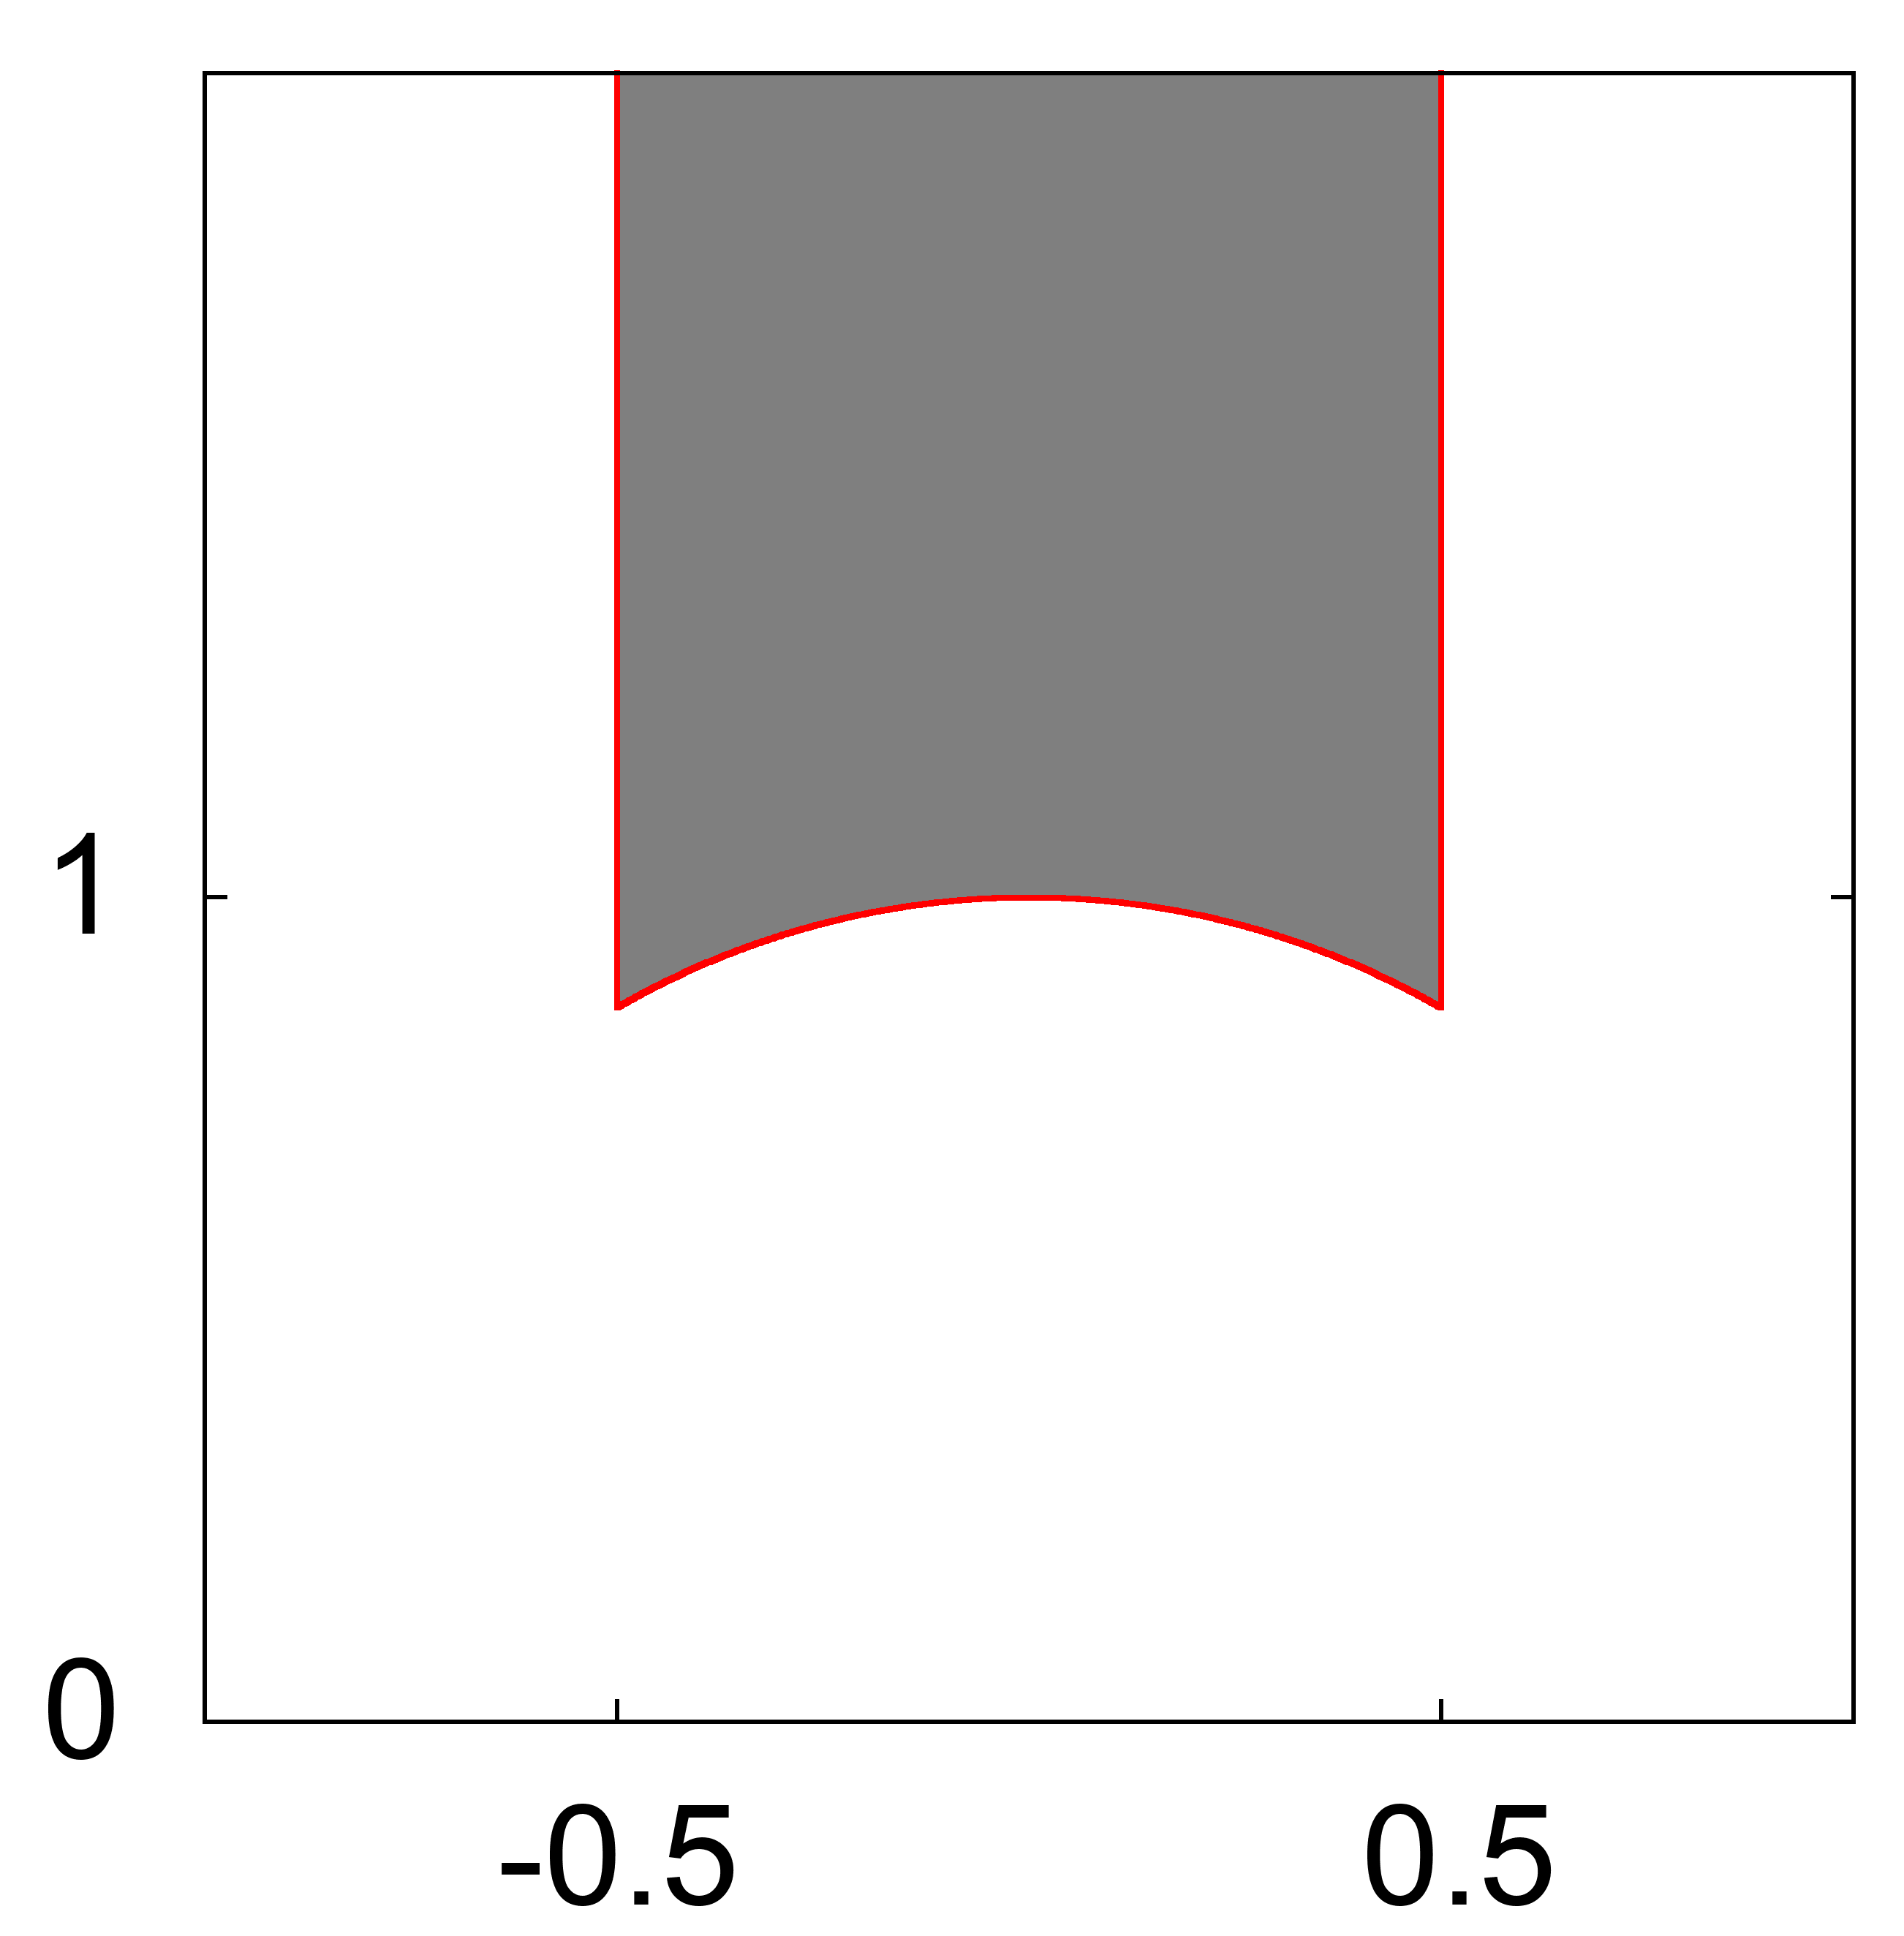
\includegraphics[width=0.5\textwidth]{fd.png}
  \end{minipage}

  Each point of $\IH$ is in the $\mathrm{SL}_2(\IZ)$-orbit of some
  (almost uniquely determined point in)
  $\cF$.  
  
  Note $\tau\in \cF \Rightarrow |q| \le e^{-\pi \sqrt{3}}<1$ and $|\mathrm{Re}(2\pi
  i \tau)| \le \pi$. 

  $\Rightarrow j|_{\cF}$ is definable in $\IRanexp$. 
\end{frame}

\begin{frame}
  Consider the product $(\tau_1,\tau_2)\mapsto
  (j(\tau_1),j(\tau_2))$ which we also denote by
  $j\colon\IH^2\rightarrow\IC^2$. We find that
  $j|_{\cF^2}\colon \cF^2\rightarrow\IC^2=Y(1)^2(\IC)$ is definable in $\IRanexp$.

  Let $V \subset Y(1)^2$ be the zero locus of $P\in \IC[X,Y]\ssm\IC$. 
  Then 
  \begin{equation*}
    j|_{\cF^2}^{-1}(V(\IC)) = \{(\tau_1,\tau_2)\in\cF^2 :
    P(j(\tau_1),j(\tau_2))=0\} 
  \end{equation*}
  is definable in $\IRanexp$ with $\dim j|_{\cF^2}^{-1}(V(\IC)) =
  2$.  
\end{frame}

\begin{frame}{Conclusion}
  \begin{itemize}
  \item O-minimal structures generalize real semi-algebraic sets
  \item There is a well-behaved dimension theory (and much more!)
  \item We need to  ``sacrifice'' wild sets like the Cantor set
    but also sets like $\IZ$ 
  \end{itemize}
  
  The most important o-minimal structures for us are:
  
  \begin{itemize}
  \item $\IRalg$ the real semi-algebraic sets
  \item $\IRan$ generated by real analytic functions restricted to
    $[0,1]^m$. This structure is useful in the context of abelian
    varieties and the Manin--Mumford Conjecture.
  \item $\IRexp$ generated by $\exp \colon \IR\rightarrow\IR$
  \item $\IRanexp$ generated by $\IRan$ and $\exp \colon
    \IR\rightarrow\IR$. This o-minimal structure is useful 
    for the Andr\'e--Oort Conjecture.       
  \end{itemize}  
\end{frame}

\begin{frame}
  \begin{center}
    Thanks for your attention.

    See you tomorrow when we apply o-minimal geometry to study
    functional transcendence.
  \end{center}
\end{frame}

\end{document}
